\documentclass[10pt,twocolumn,letterpaper]{article}

\usepackage{statcourse}
\usepackage{times}
\usepackage{epsfig}
\usepackage{graphicx}
\usepackage{amsmath}
\usepackage{amssymb}

% Include other packages here, before hyperref.

% If you comment hyperref and then uncomment it, you should delete
% egpaper.aux before re-running latex.  (Or just hit 'q' on the first latex
% run, let it finish, and you should be clear).
\usepackage[breaklinks=true,bookmarks=false]{hyperref}


\statcoursefinalcopy


\setcounter{page}{1}
\begin{document}


%%%%%%%%%%%%%%%%%%%%%%%%%%%%%%%%%%%%%%%%%%%%%%%%%%%%%%%%%%%%%%%
% DO NOT EDIT ANYTHING ABOVE THIS LINE
% EXCEPT IF YOU LIKE TO USE ADDITIONAL PACKAGES
%%%%%%%%%%%%%%%%%%%%%%%%%%%%%%%%%%%%%%%%%%%%%%%%%%%%%%%%%%%%%%%



%%%%%%%%% TITLE
\title{Arranging an Audio Track to other Genres\\
       by using CycleGAN-based Deep Learning Model 
       \thanks{Project proposal for Spring 2020, University of Wisconsin-Madison
               STAT453 Introduction to Deep Learning and Generative Models course (Instructor: Sebastian Raschka);\\
               All authors contributed equally}
}

\author{Alex DongHyeon Seo\\
{\tt\small dseo22@wisc.edu}
\and
Hyecheol (Jerry) Jang\\
{\tt\small hyecheol.jang@wisc.edu}
\and
Stella Kim\\
{\tt\small ykim736@wisc.edu}
}

\maketitle
%\thispagestyle{empty}



% MAIN ARTICLE GOES BELOW
%%%%%%%%%%%%%%%%%%%%%%%%%%%%%%%%%%%%%%%%%%%%%%%%%%%%%%%%%%%%%%%


%%%%%%%%% ABSTRACT
\begin{abstract}
  Changing the genre of a song is one of the methods used when compositing music.
  To the best of our knowledge, musicians usually add their new ideas to the song,
  while trying to keep most of the special characteristics of the original song when arranging music.
  Similar to other artistic tasks that require human creativity,
  converting the genre of a song takes a significant amount of time and effort.
  In this project, we propose a method to translate a music genre by using machine-learning,
  which can generate a new song with comparably less amount of time than humans.
  Specifically, we utilized cycleGAN based model to translate a soundtrack to another soundtrack.
  \par
  Due to the complexity and difficulties of dealing with audio data,
  our model is able to handle files written with MIDI (Musical Instrument Digital Interface) specification only with
  specific characteristics.
  In the near future,
  we expect to expand our project to use regular audio files rather than MIDI to do our tasks to generalize our model.
  By doing so, we hope our model to be used for the general public without further modifications.
\end{abstract}

%%%%%%%%% BODY TEXT
\section{Introduction}

Recent advancements of Artificial Intelligence grant computers the abilities to mimic the noble creativity of the most
intellectual lives.
One of the advancements is computer-vision which allows computers to understand images just like human beings.
However, unlike images, music has not been studied as extensive in the field of deep learning.
Thus, we thought it would be interesting to do a project using data that represent audio.
\par
Today, we are given many resources to share and access to all different types of music through apps like Spotify or
YouTube.
Due to those music apps and newly invented comfortable ear buds such as airPods, many people seem to be always listening
to music on a daily basis.
People listen to music while studying, driving, working and doing all other different types of tasks.
Because of such increasement in number of music listeners and people who are interested in music, musicians are always
trying hard to provide new musical experience to the listeners.
One of the ways that musicians create a song is changing a song to a different style of music while keeping the main
characteristics of the original song.
This is different from creating a totally new song from scratch and this way of changing a song to a new song by adding
some new ideas is called music arrangement.
Music arrangement can be done differently by making some different changes and one of the changes that could be made to
a song is the genre.
Only changing the genre of a song while keeping the main theme of the song might sound trivial but it is actually a very
difficult task which takes quite a long time and much effort.
Therefore, we would like to see if changing the genre of music could be done using machine-learning methods. 
\par
Our goal is very similar to AmazonWeb Service’s DeepComposer \footnote{
  AWS DeepComposer Product Description Page: \url{https://aws.amazon.com/deepcomposer/}
},
a keyboard that allows people to create a new song or arrange to a different genre with
a simple combination of notes of their own.
DeepComposer is based on deep learning models using generator and discriminator to update the music.
Slightly different from DeepComposer,
our project will focus on transferring the genre of the song to the user’s desired genre.


\section{Literature Review / Backgrounds}

\subsection{Audio Files}

Our initial goal was to use raw audio files to train and test our model to generate a new song with a change in the
genre of the original song.
\par
However, while trying to find any good examples of machine learning models that use binary audio files for training and 
testing, we realized that there is not a well-made model that could be used for raw audio files.
Unlike images, there are not many models that are made for audio files.
Thus, we decided to make a small change in our plan. 
\par 
Instead of using audio files directly to the model, since we could not find a model that takes audio files as input, 
we thoguht we could use a converter that translates audio files to MIDI files.
Even though we failed to find a machine learning model that uses audio files,
we were able to find some models that use MIDI files.
Because there are some models that were used with MIDI files,
we thought it would work out if we can translate audio files to MIDI files and use them to train the model. 
\par
However, we faced another difficulties.
We could not find the right converter that could be used in converting the type of file from audio such as MP3 to MIDI.
After failing to find a way to auido file directly to a machine learning model and also failing to find a good converter
that changes audio files into MIDI files,
we decided to use MIDI files and build a model that takes in MIDI files as input for training and testing. 
\par
\paragraph{MIDI Files}
MIDI file is a type of file that represents audio using binary based on 128 representations of different
instruments \cite{midiSpec}. 
Inside a MIDI file, there are instructions written in binary that describe the attributes and characteristics of the 
song.
For example, the file contains the information about the velocity of the song,
which instruments to be played at which point of the track time and any other details that are needed to make the music. 
\par
Some advantages of using MIDI files is that MIDI files specify the 128 different instruments independently.
As mentioned above, the MIDI files has their own way of representation of 128 instruments and they can be used in
various ways depending how they are written in the MIDI file.
Becuase those instruments are specifically described how they are played at which speed and time in MIDI files,
every details of the information about the instruments that make up the sound of songs could be recorded.
This is good for the purpose of our project since when generating a new song based on a song that already exists,
it is very important to keep most of the details and the main style of the song. 
\par
Therefore, having the specifications of the music is helpful in maintaining the important sounds and notes when making
a new song based off of the original version.


\subsection{Model Architecutures}
\paragraph{conditional GAN Image-to-Image Translation}
Translating a type of image to another type of image can be viewed as translating pixel by pixel of an image.
Thus, instead of having different algorithms for different types of image translation~\cite{isola2017image},
uses conditional Generative adversarial network(cGAN) to provide general solutions to any type of image translation.
For any type of image translation, the same architecture and objective are used but is trained using different paired 
image dataset through Conditional GAN by putting conditions on the input image and outputting the corresponding image.
\par
\paragraph{CycleGAN for Image-to-Image Translation}
Often finding a large size of paired dataset can be very expensive and difficult.
On the other hand, unpaired dataset can be a little more reasonable to find compared to the paired dataset.
Thus, Zhu et al.~\cite{zhu2017unpaired} provides a solution to such problem where the training samples do not have to be
paired.
Zhu et al.~\cite{zhu2017unpaired} did image-to-image translation which is translating a type of image to a different 
type using CycleGAN.
CycleGAN’s approach is that, instead of learning using paired dataset for training, 
learning from unpaired dataset of source domain X and target domain Y.
Its strategy is that given domain X, the translated version of X to domain Y type should be translated back to domain X 
type without much loss.
\par
Since it is hard to find paired dataset for arranged music,
cycleGAN's approach is more suitable for our research, compared to cGAN.


\subsection{Baseline Code}
CycleGAN can not only learn from image dataset, but also can be used to learn from different types of dataset.
One example is using CycleGAN to learn from MIDI files to do music genre transfer~\cite{brunner2018symbolic}.
This example takes advantage of the concept of domain translation of CycleGAN and applies the concept to MIDI files with
an extra discriminator to maintain the original structure of the input song.
\par
Even though the Brunner et. al’s model was great initial model that we could start based on and build upon for our
project, we found some fatal problems inside the code~\cite{brunner2018symbolic}.
The first issue we faced was the significant detail loss in training/testing files.
Because Brunner et. al. cut off, trimmed, and merged sound channels in the file under too many conditions,
it caused the files to lose a big portion of information in them~\cite{brunner2018symbolic}.
\par
The second problem was that the codes to access directories were hard coded
(the path of Brunner et. al.'s machine appears as string literals inside the code numerous times).
This caused some inconvenience while training the model using our own data,
since there were quite a lot of lines that link to the directories where data was stored.
Therefore, we had to fix the code to generalize the directory access instead of having to change and type multiple lines
of code to access the directory of data every single time.
\par
The last problem was the version and update issues.
The code was written in Tensorflow 1.4 and has not been updated to the newest version.
This arose as an issue because Tensorflow 1.4 is too old and is not supported on various platforms anymore.
Specifically the tool we used, called Colab, does not support Tensorflow 1.4 anymore,
but changing the code to Tensorflow 2, which is the newest version of Tensorflow,
was such a challenging task since those two versions are too different.
Thus, we changed the code into Tensorflow 1.15 which is the newest version of Tensorflow 1.


\section{Proposed Method}

% TODO
% Describe the method(s) you are proposing, developing, or using. I.e., details
% of the algorithms may be included here. 

\section{Experiments}

We generated two version of model to proof our idea.
The first model utilizes the original soundtrack without any filteration or merging.
The second model we tried merges all the channels in MIDI file to one track (representing the piano's sound).
\par
All the model follows the basic structures that proposed on Brunner et. al. \cite{brunner2018symbolic}.
For the second model, we tried four different settings during the training time.
The first setting uses learning rate of 0.0002,
epoch of 100 and second setting uses learing rate of 0.0001 and epoch of 200.
The first and second setting uses 64 convolution filters on generator.
For the third and fourth setting the learning rate and the epoch numbers are identical to the first and second setting, 
but it uses 128 convolution filters on generator. 


\subsection{Dataset}

Finding a large amount of music having paired labels(the arranged/mixed music based on the same track) is very
challenging and even considered as impossible task, since there is a limited number of arranged tracks for each
music(with high possibility, there is no arranged track).
To use cycleGAN~\cite{zhu2017unpaired}, we at least need to have unpaired labeled data.
More specifically, we need music sources which have genre information as their label.
Also, because the music industry is one of the most sensitive markets toward copyright issue,
it is also important to only use the music tracks which do not have any restrictions on the usage for research purposes.
\par
\paragraph{Data Collection}
For this project, we collected MIDI files of different genres, including Classical, Pop, Rock, and Jazz.
We first tried collecting MIDI files of all four different genres from the same database to ensure the fairness and
equality across all the files; however, we could not find a good database that has good MIDI files of all the four
genres we intended to use for the project.
Thus, we allowed ourselves to collect the files of each genre from different databases.
At the end, we collected MIDI files of classical music from mfiles\footnote{
  Classical Database: \url{https://www.mfiles.co.uk/classical-midi.htm}
}
while MIDI files of Pop and Rock are from midiworld \footnote{
  Pop Database: \url{https://www.midiworld.com/search/?q=classic} \linebreak
  Rock Database: \url{https://www.midiworld.com/search/?q=rock}
}.
However, we had some difficulties finding a good set of MIDI files of Jazz music so we used the same data with
Brunner et al. \cite{brunner2018symbolic} 
\par
For classical, pop and rock MIDI files, we did data crawling since those files are from websites.
To do data crawling, we first used import.io, \footnote{
   Import.io product website: \url{https://www.import.io/}
}
which is a web application that gets all the text contents of a webpage including links.
Then we used R to cut off all the unnecessary text data we got from import.io to only select the download
links for files.
After cleaning up the data, then we used for-loop in R to go through the iterations and download all the files that are
linked to addresses that we found earlier.
For Jazz, we simply downloaded the files from GitHub.
\par
\paragraph{Dataset Analysis}
After we downloaded the MIDI files, we manuver over the collected data to be more familiarized with those.
At a glance, as the MIDI files are usually generated by the amateurs, rather than officially released from professonal
entertainment companies, they are not well-organized.
For instance, Some of them contain meaningless trailing and ending whitespaces rather than their first note appears at
time 0.
\par
Moreover, as there exists the genres having characteristics from more than one genre
(for instance, pop rock has characteristics from both pop and rock musics),
it is hard to tell which musics belongs to which genre for some soundtrack.
Also, the existence of variations in one genre
(for example, inside of the rock genre, we have hard rock, progressive rock, punk rock and so on)
made us hard to pin-point the specific characteristics that each genre has.
However, as there is no available databases such that categorizes the MIDI files in very specific genres,
we decide to stay on using the big genre classes.
\par
\paragraph{Data Pre-Processing}
Due to the unstructuredness of the retrieved dataset, we are forced to preprocess the data.
During the data preprocessing, the baseline code dropped the songs which have time signature change,
of which the first beat does not start at time zero, and of which time signature is not 4/4 \cite{brunner2018symbolic}.
The filter that Brunner et. al used is implemented in a very precise and specific way,
which makes the songs that go through the filter ruins the song in such way that the music does not represent the 
intended genere anymore.
\par
For the first experiment to make the model more generalized, we removed those filters before we processed the data.
For the second experiment, which merges all the sound channels into one channel, we removed the trailing and ending
whitespaces so that it can minimize the blank audio slices after cutting the sound to fixed-length slices.


\subsection{Software}

The baseline code was written in TensorFlow 1.4, which is very out-dated.
We updated code so that it is at least runs without any warning or errors on the latest TensorFlow 1.x.
As of now, though the TensorFlow 1 is outdated, we decided to use TensorFlow 1 as we are more familiar to.
\par
To read and manipulate MIDI files properly, we utilizes pretty\textunderscore midi \footnote{
  pretty\textunderscore midi Documentation: \url{http://craffel.github.io/pretty-midi/}
}
and Pypianoroll \footnote{
   Pypianoroll Documentation: \url{https://salu133445.github.io/pypianoroll/}
}.


\subsection{Hardware}

For local testing before uploading the code and start train our model,
we used Dell XPS 9550, which equipped Intel's i7-6700HQ @ 2.6Ghz, DDR4 2133Mhz,
and NVIDIA GeForce GTX 960M with vRAM of 2GB.
\par
After testing locally, for our main training, we used Google's Colaboratory Pro.
We used standard instance (runtime),
which have 12GB of RAM with NVIDIA NVIDIA Tesla P100 Graphic Cards having vRAM of 16GB.
\par
Note that we continuously encountered with IOError while we training models on CoLab.
It was because the mounted Google Drive timeout while the colab computing instance tries to access to the saved
pre-processed training data.
To fix this issue, we first lookup the list of files/directories that is used while training,
and then run the training codes.
It is mainly because the CoLab instance does not copy and save all the contents in the google drive to its local path,
and it takes time (probably network transferring time) to retrieve massive amount of training data at once.
\par
Not only we encountered the issue while loading training data, we also encountered problem while saving data back to the
drive from the CoLab instance.
The CoLab instnace messaged us that it successfully saved the files to the drive path, but when we open the drive,
there does not exist the files that we expected to see.
This is becuase the files that we tried to save is stored in the local disk space of the CoLab Instance,
rather thanflushed directly back to the network location.
To solve this issue, Google implemented a new function called flush\textunderscore and \textunderscore unmount()
to ensure whether all the information that locally saved has been syncronized to the drive or not.
In other words, to gaurantee the local data to be syncronized with the network space, you should call
flush\textunderscore and \textunderscore unmount() before you terminate the session.


\section{Results and Discussion}

To summarize, we obtained two different results from the first version of our model, which is the generalized model,
and the second version of our model, which is the model with merged channel.
The first version of our model was based on the model that was prposed on Brunner et. al. \cite{brunner2018symbolic},
we modified the model by removing filters and made generalized model.
The reason why we removed the filter from our model is that, 
model that was proposed on Brunner et. al. \cite{brunner2018symbolic} had filter for the MIDI file to have 
time signature chages, remove songs that does not start at time zero, and remove songs that do not have time signature 
of 4/4.
By using this filter we thought that music that goes in to the model will be too specific, therefore, the filtered songs
will not represent the genre as a whole.
Since our main goal is to detect the characteristics of the song's genre and generate new composed song with different 
genre from given input data, we decided to make a more generalized model for our first trial.
\par
The genre change we first tried with our generalized model was pop song to classical song and classical song to pop song.
However, both of the outputs that were generated from our generalized model were not successful.
The generated songs sounded like it did not have any similarity with the original song, and consisted with random notes.

You can see the visualization of the MIDI file based on example results from generalized model that we used for the presentation 
shown in Figure \ref{fig:Image1} and Figure \ref{fig:Image2}.

\begin{figure*}
  \begin{center}
     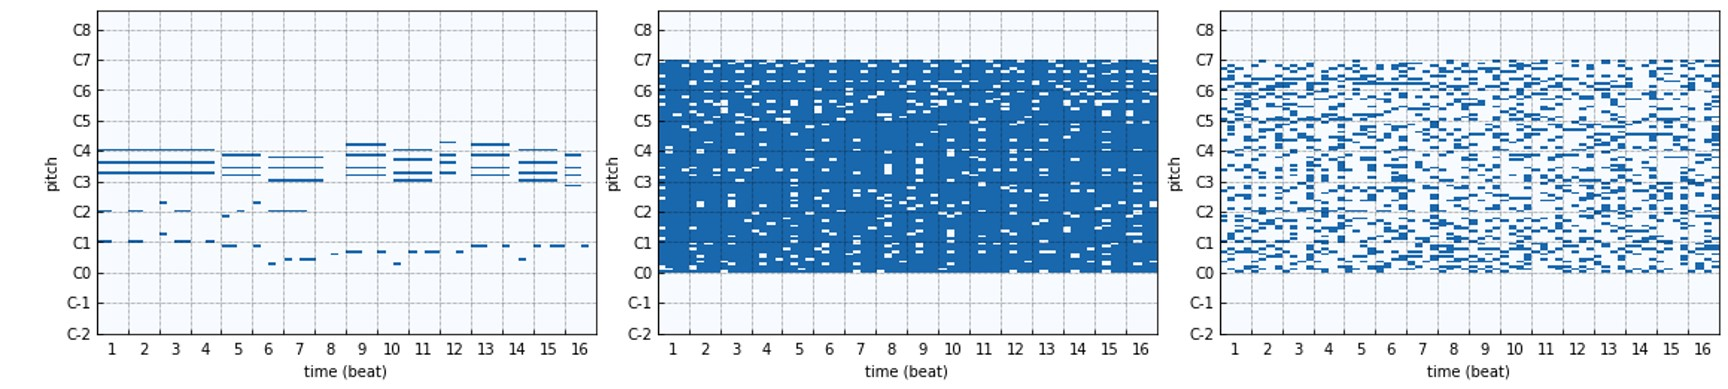
\includegraphics[width=0.8\linewidth]{figures/Image1.jpg}
  \end{center}
     \caption{Example output of visualizaion for MIDI file from Generalized model, pop song to classical song.
      Origianal-Transferred-Cycle, in that order}
  \label{fig:Image1}
  \end{figure*}

  \begin{figure*}
    \begin{center}
       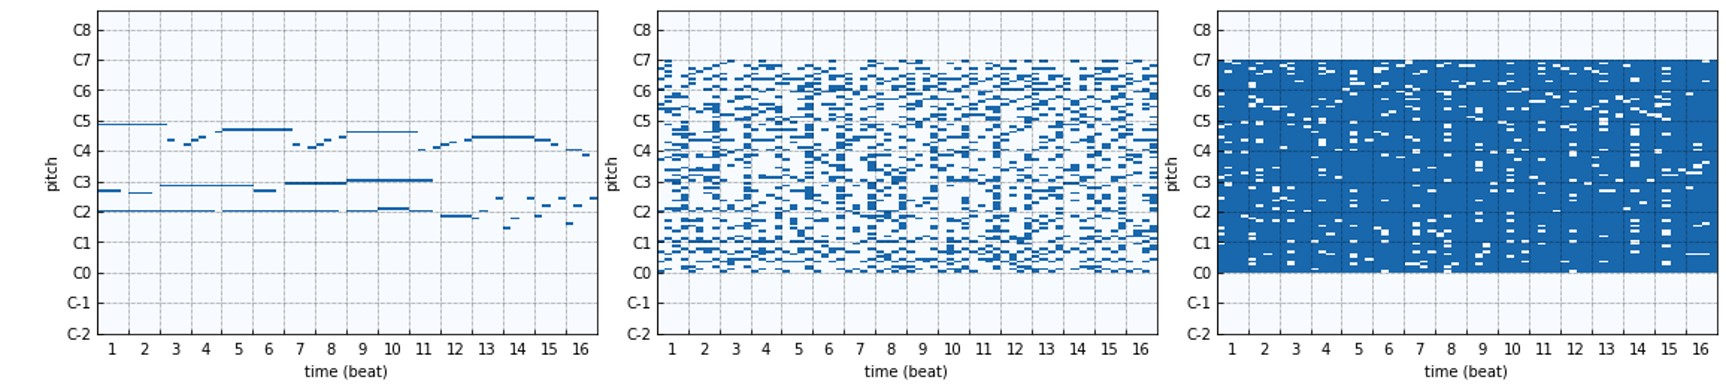
\includegraphics[width=0.8\linewidth]{figures/Image2.jpg}
    \end{center}
       \caption{Example output of visualizaion for MIDI file from Generalized model, classical song to pop song.
        Origianal-Transferred-Cycle, in that order.}
    \label{fig:Image2}
    \end{figure*}
To solve the problem, we analyzed our code and tried to find out the problem and fix it.
From our analysis,
we figured out that original songs that were used, which is the song that we are trying to transfer to different genre,
did not contain all sounds as the code only used one track,
in our case piano, and dropped the others such as drum, bass and guitar.
The reason why our code only used one track was that our model only accepted 2D array, [tone, time] for training, 
which was more suitable for the piano.
Hence, our model choosed to use piano as a single track.
Another problem that we found was that our input data did not represent all the sounds of a song.
For example, in pop song, besides the sounds from different instruments, such as piano and guitar,
there is also a melody from vocal that contributes to the sounds of a song.
Since the MIDI file does not provide the melody or sound of the vocal,
it was hard for our data to represent all the sounds of the song.
These problems that we found were causing the our generalized model unable to learn the characteristics of each genre,
hence, the unsuccessful output with random notes.
\par
The second version of our model we revised our first generalized model to fix the discovered problems.
One of the solutions that we came up with was merge tracks to solve dimension,
and the other solution was to fix the code to utilize the 3D tensor for input,
in order to represent all the sounds of different instruments from the song.
Considering difficulties and efficiency to fix the problem, we decided to merge tracks to one channel.
Additionally, we tried to remove trailing and ending whitespace from the MIDI file before slicing to fix the empty blank
slices of the MIDI file.
After fixing main problems, we made four different models with diffferent hyperparameters.
We set the first and second model with 64 convolutional filters for the generator,
while setting third and fourth model with 128 convolutional filters for the generator.
In the case of epoch and learning rate, first model was set with 'epoch=100' and 'Learning Rate = 0.0002'.
Second model was set with 'epoch=200' and 'Learning Rate = 0.0001'. 
Then, for the third model, epoch and learning rate was set with 'epoch=100' and 'Learning Rate = 0.0002'.
Fourth model was set with 'epoch=200' and 'Learning Rate = 0.0001'.
However, our third and fouth model have failed on training due to errors from Google CoLab. 
To summarize, first and second model was successful on training phase while the learning rate linearly diminished after
50\% of epoch.

You can see the visualization of the MIDI file based on example results from merged channel model that we used for the presentation 
shown in Figure \ref{fig:Image3}, Figure \ref{fig:Image4}, Figure \ref{fig:Image5}, and Figure \ref{fig:Image6}.

\par
% TODO FIGURE 3, 4, 5, 6
\begin{figure*}
  \begin{center}
     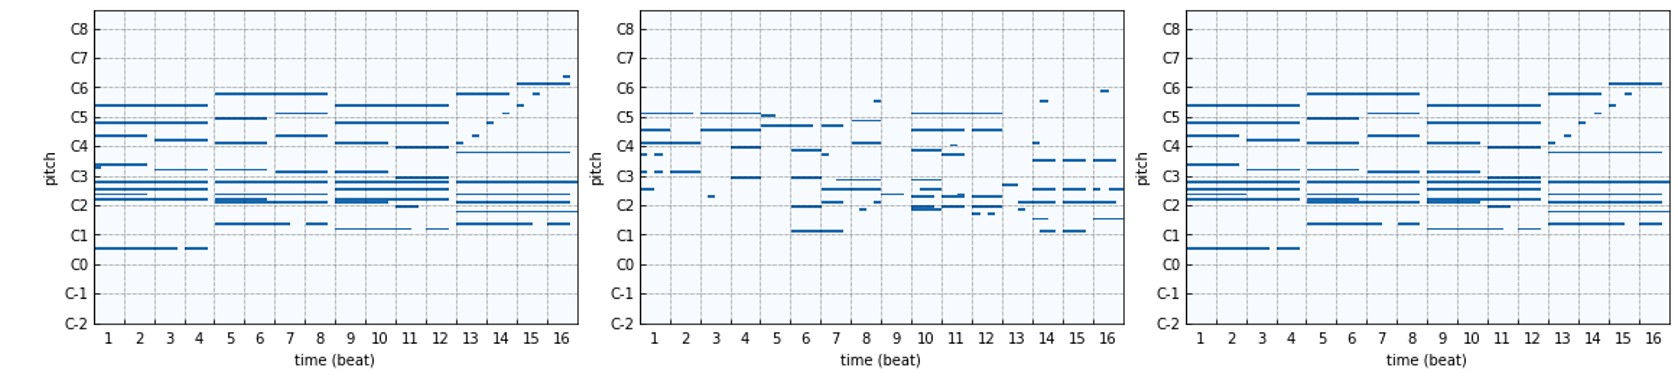
\includegraphics[width=0.8\linewidth]{figures/Image3.jpg}
  \end{center}
     \caption{Example output of visualizaion for MIDI file from First Merged channel model, pop song to classical song.
      Origianal-Transferred-Cycle, in that order.}
  \label{fig:Image3}
  \end{figure*}

  \begin{figure*}
    \begin{center}
       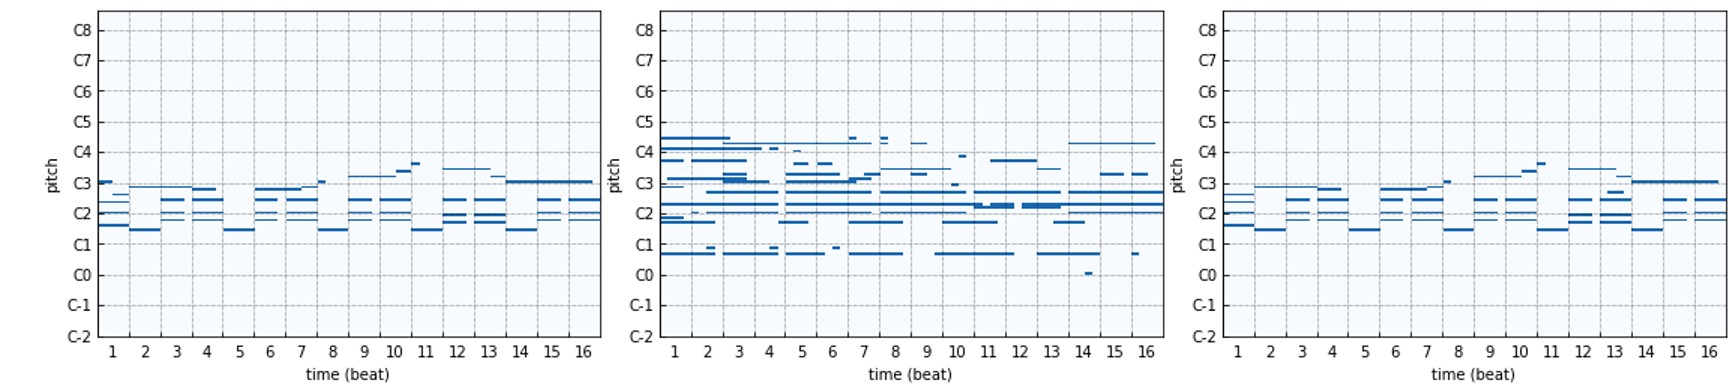
\includegraphics[width=0.8\linewidth]{figures/Image4.jpg}
    \end{center}
       \caption{Example output of visualizaion for MIDI file from First Merged channel model, classical song to pop song.
        Origianal-Transferred-Cycle, in that order.}
    \label{fig:Image4}
    \end{figure*}

    \begin{figure*}
      \begin{center}
         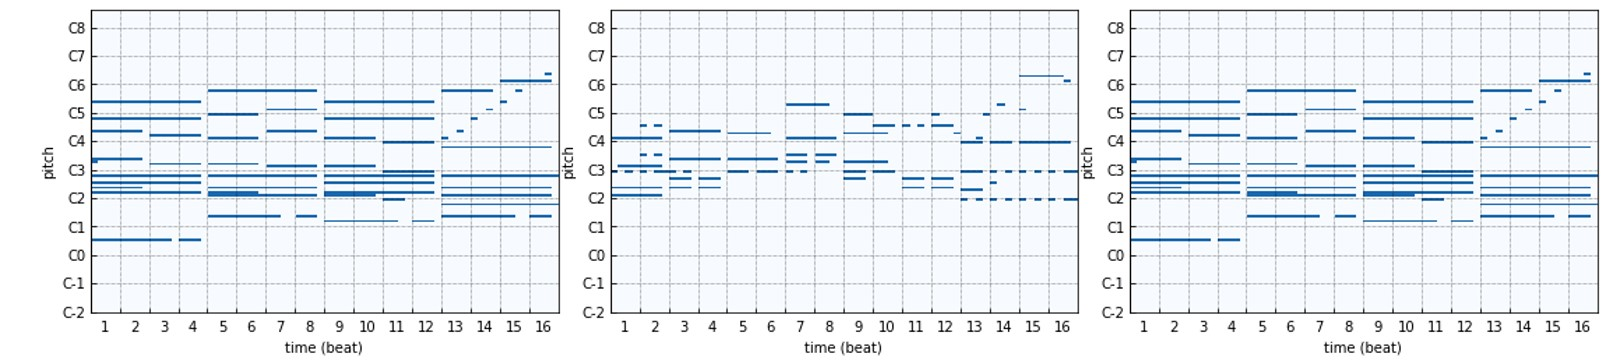
\includegraphics[width=0.8\linewidth]{figures/Image5.jpg}
      \end{center}
         \caption{Example output of visualizaion for MIDI file from Second Merged channel model, pop song to classical song.
          Origianal-Transferred-Cycle, in that order.}
      \label{fig:Image5}
      \end{figure*}

      \begin{figure*}
        \begin{center}
           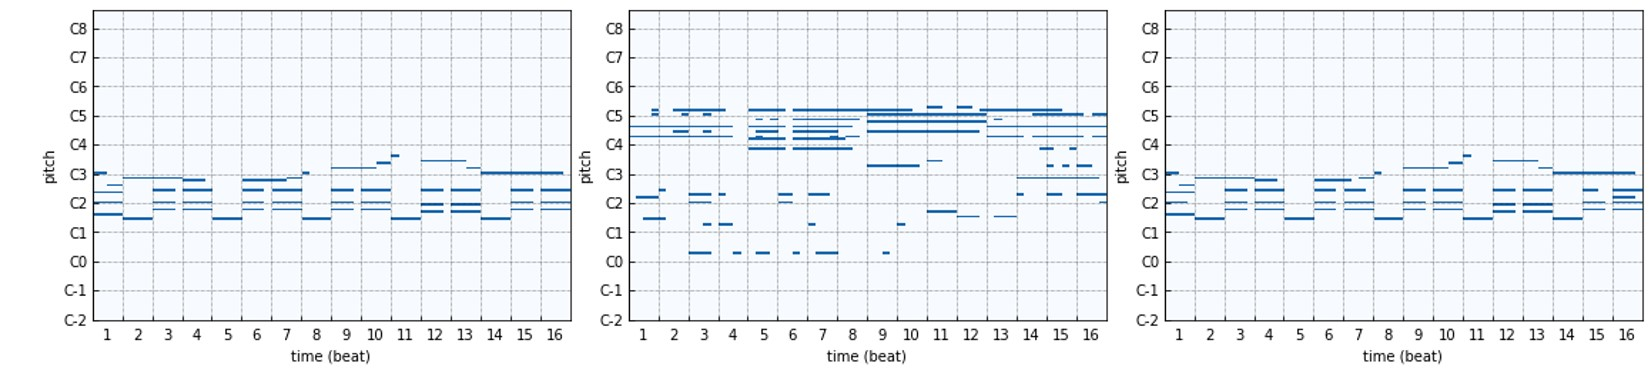
\includegraphics[width=0.8\linewidth]{figures/Image6.jpg}
        \end{center}
           \caption{Example output of visualizaion for MIDI file from Second Merged channel model, classical song to pop song.
            Origianal-Transferred-Cycle, in that order.}
        \label{fig:Image6}
        \end{figure*}
The genre change we tried with our two models with tracks being merged in to one channel,
was same as what we did with our first generalized model, pop song to classical song and classical song to pop song.
The outputs that were generated from our model was much more successful compared to our first generalized model.
It did not sounded like song with random notes like first outputs,
but sounded similar to the original songs that were given.
Our outputs contained the melody from the original songs that were given,
but sounded differently as if the genre was changed like we intended to.
However, since the outputs only contained piano based melody,
it was hard to distinguish if the genre of the song was pop or classical.
However, the songs that were transferred to classical song from pop song contained much more harmonical sounds
than the original songs, just like normal classical songs.
For the songs that were transferred to pop song from classical songs, 
they contained less harmonical sounds than the original songs,
but contained experimental melody than the origianl songs, just like normal pop songs.
\par
From our results, we have noticed that the problem of our outputs not being significant
as we intended to be might coming from various reasons.
We discussed that it is possible that lots of pop songs are already motivated from classic songs, therefore,
we could not listen significant difference between generated songs and original songs and easily notify their genres.
Another point that we have discussed is that by removing various instrument information,
it ruins the characteristics of each genre.
Additionally, we realized that there is no perfect way to pass full audio information to deep learning model.
While we used MIDI file for our input data, normally, MIDI file is not generalized approach to represent music.
We also realized that, while the ResNet and U-Net are reckoned to be the state-of-the arts convolution filters
for vision tasks,
there was no adequate and appropriate convolutional filter for audio tasks to the best of our knowledge.


\section{Conclusions}

In this project, we presented two different models to generate songs with transferred genre of the given songs.
While our first model that was generalized by removing filter from model that was prposed on
Brunner et. al. \cite{brunner2018symbolic}, did not give us satisfying result,
our second model that we revised from the first model by merging tracks into one channel gave us better results.
While our results from first model did not sound like song with consisting of random notes,
results from the second model showed similarity with given original songs and composed the song to
the intended genre in someway.
We mostly worked on analyzing related work, revising code, and preprocessing the data, 
since applying deep learning with audio data is not much developed yet compared to computer vision field.
From ananlyzing the models and codes,
we found out existing problems and discussed how we could improve our model to generate convincing songs.
While our final result can be confusing for normal audience to realize if the genre has been changed,
we are satisfied with our results. 
\par
From deep discussions, we found out some possible improvements that could be made for the further studies.
The results can be more significant by trying our models for other genre,
such as jazz and rock rather than pop and classical.
Additionally, we could modify the model structure to get 3D tensor as an input to represent
all the instruments from the song, so that it could represent their genre better.
We also discussed about using spectogram to deal with this complicated audio tasks,
while it could be hard to map the spectogram back to audio, it coul be useful for the classification of the genre.


\section{Acknowledgements}

Our project is part of Spring 2020 semester's Statistics 453 \footnote{
  Course Website: \url{http://pages.stat.wisc.edu/~sraschka/teaching/stat453-ss2020/} \linebreak
  GitHub Repository: \url{https://github.com/rasbt/stat453-deep-learning-ss20}
}
(Introduction to Deep Learning and Generative Models) course of the University of Wisconsin-Madison.
We specially appreciate with Prof. Raschka for all of his effort toward lectures and support toward our project.


\section{Contributions}

All of our team member decide to work on all steps and tasks together,
as we believe it is important for everyone to at least understand how and what we are doing to achieve the common goal.
However, as each individual has his/her own specialties and strength, some tasks has been designated to specific person.
\par
As Hyecheol (Jerry) Jang has strength on understanding and fixing the codes written on python,
he mainly worked on analyzing and fixing the baseline code.
To do so, he went through the tensorflow API to understand what's going on inside the code and to remove depressed and 
unsupported code parts from the baseline code.
\par
Alex studied similar studies and papers that are about creating music in various ways.
He did research on the papers to find out which method worked and why specific methods worked better than the others.
Also, he reviewed different models to find out which model would fit the best for the purpose of project. 
\par
Stella worked on finding the right MIDI files for the project.
She went through various websites and databases to select the correct MIDI files that could be used for the purpose of
our project.
Also, she worked on understanding the code of the baseline model for the data processing part,
to understand why the data was processed in such way, she had to study the MIDI file characteristics and music as well.
\par
Even though we had some specific tasks assigned to each person,
overall, as mentioned above, we helped each other and worked togehter on most of the tasks.
Also, we divided the work on the presentation and the report evenly as well.


\section{Codes}

All the codes are posted on the GitHub repository. \footnote{
   \url{https://github.com/hyecheol123/CycleGAN-Music-Style-Transfer}
}
The repository ipynb file that used as an interactive workspace to run the code.
All the data preprocessing codes are embedded on the notebook as we want to run those code only when needed.
The model has been implemented in the python files, and it is called inside the notebook.


{\small
\bibliographystyle{ieee}
\bibliography{bibliography.bib}
}

\end{document}
